\documentclass{replab}
\usepackage{lipsum}
\usepackage[shortlabels]{enumitem}
\usepackage{amsmath}
\usepackage{physics}
\usepackage{bm}

% --- Información del documento ---
\title{Taller - Semana 7}
\author{Diego Alejandro Heredia Franco}

% Nota: Si se desea incluir más de un autor en el documento, el archivo replab.cls, en la sección "Página de título de documento", contiene líneas de código comentadas pensadas para introducir los datos desde 1 hasta 4 autores. Sin embargo, debe escogerse solo una de las cuatro secciones de código y comentar las demás para mantener la consistencia del documento.

\date{14/15 de mayo de 2025}
\subtitle={Cinemática No. 2}
\email={\href{mailto:dherediaf@unal.edu.co}{\color{principaluno}\texttt{dherediaf@unal.edu.co}}}
\subject={Taller Fundamentos de Mecánica}

\setlength{\columnsep}{14pt}

% --- Archivo de bibliografía ---
\addbibresource{repbib.bib}

% --- Inicio del documento ---
\begin{document}
\setlength{\parindent}{0pt}
	
	\pagestyle{fancy}
	\unspacedoperators
	
% --- Título ---
	{\begin{tcolorbox}[colframe=white, colback=principaldos, arc=8pt]
		\begin{center}
			\maketitle
			%\rule{\textwidth}{0.2pt}
			%\medskip

			%\noindent\textit{Palabras Clave:} medidas directas e indirectas, análisis estadístico, incertidumbre, calibrador Vernier, balanza.
		\end{center}
	\end{tcolorbox}}
	\selectlanguage{spanish}

	Los ejercicios que aquí se presentan, han sido tomados de \cite{lanaturaleza}, \cite{serway}, \cite{londono} y \cite{sears} en los capítulos relacionados con cinemática y movimiento rotacional.\\

{\begin{tcolorbox}[colframe=red!50!black, colback=red!5!white, arc=8pt]
	\textbf{\textcolor{red!50!black}{Sugerencia:}} En el libro \textit{Física Universitaria Vol.1} (Zemansky) \cite{sears}, se presenta al final de cada sección un \textit{\textbf{resumen de los conceptos más importantes}}, así como un pequeño manuscrito con una \textit{\textbf{estrategia para resolver problemas}}. Se recomienda al estudiante leer este instructivo para que pueda resolver los ejercicios de forma más organizada y eficiente.
\end{tcolorbox}}

% --- Cuerpo del reporte ---
\section{Introducción al Movimiento Rotacional}

\subsection{Cinemática en Coordenadas Polares \textcolor{red}{*}}

La posición de un objeto $\vec{r}(t)$ descrita en coordenadas cartesianas se escribe como se observa en la (Eq. \refeq{eq:posicion}). Teniendo en cuenta la relación entre coordenadas cartesianas y polares\footnote{$x = r\cos(\phi)$, $y = r\sin(\phi)$, y $\phi$ es el ángulo asociado al vector de posición medido desde el eje x en dirección contraria a las manecillas del reloj.}. Exprese la a) posición, b) velocidad y c) aceleración del objeto en coordenadas polares e identifique en cada caso d) la velocidad y aceleración: tangencial, normal y angular.
\begin{align}
	\vec{r}(t) = x(t)\hat{\imath} + y(t)\hat{\jmath}
	\label{eq:posicion}
\end{align}

\textit{\textbf{Nota:}} Recuerde que a diferencia de las coordenadas cartesianas, en coordenadas polares los vectores unitarios de posición $\hat{r}$ y $\hat{\phi}$ dependen del ángulo $\phi$ y por lo tanto no son constantes.

\subsection{Movimiento Circular Uniforme}
Un objeto se mueve en una trayectoria circular de radio $r$ con \textit{rapidez} constante $v$. a) Determine la velocidad y aceleración centrípeta\footnote{En movimiento circular, la aceleración centrípeta es el nombre que se le da a la aceleración normal que es perpendicular a la velocidad tangencial.} y tangencial del objeto en función de $r$ y $v$.\\ 

¿Cuál es el valor de la velocidad y aceleración angular en función de $r$ y $v$? b) Determine en analogía con el movimiento rectilíneo uniforme las ecuaciones que describen el cambio del ángulo $\phi(t)$ en función del tiempo. Con esta información determine el periodo de oscilación $T$.\\

\subsection{Movimiento Circular Uniformemente Acelerado}
	Un objeto se mueve en una trayectoria circular de radio $r$ con aceleración angular $\alpha \neq 0$. a) Determine la velocidad y aceleración centrípeta y tangencial del objeto en función de $r$ y $\alpha$. b) En analogía con el movimiento rectilíneo uniformemente acelerado, determine el valor de la velocidad angular $\omega(t)$ y el ángulo $\phi(t)$ en función del tiempo.

\section{Movimiento Rotacional}

\subsection{Disco y Masa Colgante}
Un disco  $D$ (Fig. \ref{fig:disco}) está rotando libremente alrededor de su eje horizontal. Una cuerda esta enrollada alrededor de la circunferencia del disco, y un cuerpo $A$, unido a la cuerda, cae bajo la acción de la gravedad. El movimiento de $A$ es uniformemente acelerado pero su aceleración es menor que la de la gravedad. Cuando $t=0s$ la velocidad del cuerpo $A$ es $0.04m/s$, y dos segundos más tarde $A$ ha caído $0.2m$. Encontrar las aceleraciones tangencial y normal, en cualquier instante, de un punto cualquiera del borde del disco.

\begin{figure}[htbp]
	\centering
	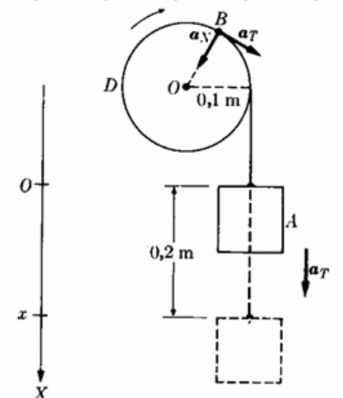
\includegraphics[width=.2\columnwidth]{imagenes/disco.png}
	\caption{Dibujo esquemático del disco y la masa colgante.}
	\label{fig:disco}
\end{figure}

\subsection{El Carrusel}
a) ¿Cuál es el periodo y velocidad de una persona en un carrusel, si la persona experimenta una aceleración de magnitud $0.80m/s^2$ cuando esta a $4.0m$ del eje de rotación? b) ¿Cuál es la magnitud de la aceleración y la velocidad si ahora la persona se ubica a $2.0m$ del centro del carrusel? Asuma que el carrusel se mantiene rotando con el mismo periodo.
	
\subsection{Centrifuga de Laboratorio}
\textbf{Aplicación Biológica} 

La sangre humana contiene plasma, plaquetas y glóbulos rojos. Para separar el plasma de los otros componentes, se utiliza la centrifugación. Una centrifugación efectiva requiere someter la sangre a una aceleración de $2000g$ o más. En este caso, se asume que la sangre está contenida en tubos de ensayo de $15cm$ de largo y completamente llenos de sangre. Estos tubos giran en la centrífuga inclinada a un ángulo de $45^\circ$ por encima de la horizontal (Fig. \ref{fig:centrifuga}).

% Para hacer un espacio dentro de una ecuacion se utiliza \,

\begin{enumerate}
	\item[a)] ¿Cuál es la distancia de una muestra de sangre al eje de rotación de una centrífuga que gira a $3500\,\text{rpm}$, si tiene una aceleración de $2000g$?

	\item[b)] Si la sangre en el centro de los tubos gira alrededor del eje de rotación a la distancia calculada en el apartado (a), calcula las aceleraciones que experimenta la sangre en cada extremo del tubo de ensayo. Expresa todas las aceleraciones como múltiplos de $g$.
\end{enumerate}


\begin{figure}[htbp]
	\centering
	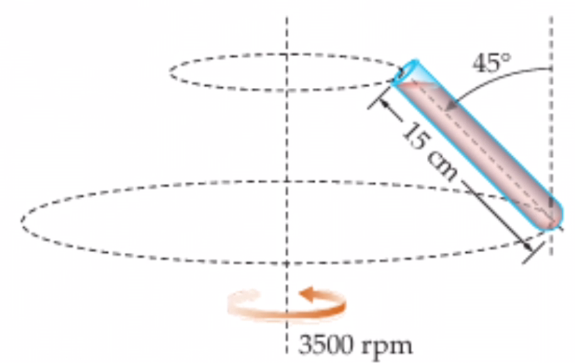
\includegraphics[width=.4\columnwidth]{imagenes/centrifuga.png}
	\caption{Dibujo esquemático de la centrifuga de laboratorio.}
	\label{fig:centrifuga}
\end{figure}
	

\subsection{Entrenamiento de Astronautas}
Conforme se separan los cohetes propulsores, los astronautas del transbordador espacial sienten una aceleración de hasta $3g$, donde $g = 9.80\,m/s^2$. En su entrenamiento, los astronautas montan un dispositivo en el que experimentan tal aceleración como una aceleración centrípeta. En específico, el astronauta se sujeta con firmeza al extremo de un brazo mecánico que luego gira con rapidez constante en un círculo horizontal Determine la rapidez de rotación, en revoluciones por segundo, requerida para dar a un astronauta una aceleración centrípeta de $3.00g$ mientras está en movimiento circular con radio de $9.45\,\text{m}$.


\subsection{Vector Aceleración}
Un automóvil de carreras parte del reposo en una pista circular; aumenta su rapidez a una cantidad constante $a$, conforme da una vuelta a la pista. Encuentre el ángulo que forma la aceleración total del automóvil, con el radio que conecta el centro de la pista y el auto, en el momento en que el automóvil completa el círculo.

\subsection{Tren Frena en una Curva}
Un tren frena mientras entra a una curva horizontal cerrada, y frena de $90.0\,\text{km/h}$ a $50.0\,\text{km/h}$ en los $15.0\,\text{s}$ que tarda en cubrir la curva. El radio de la curva es de $150\,\text{m}$. Calcule la aceleración en el momento en que la rapidez del tren alcanza $50.0\,\text{km/h}$. Suponga que continúa frenando a este tiempo con la misma relación.

\subsection{Partícula en Movimiento Circular Uniforme}
Una partícula se mueve alrededor de un círculo de radio $r = 0.14\,\text{m}$ en el plano $x$–$y$. Su rapidez angular es de $\omega = 3.7\,\text{rad/s}$. Cuando $t = 0s$ pasa por el eje $x$. (El origen está en el centro del círculo.) Determine las ecuaciones para la posición, velocidad y aceleración de la partícula cuando $t = 0.40\,\text{s}$ y $t = 1.3\,\text{s}$.

\subsection{Partícula en Movimiento Circular Frenando}
Un disco que rota alrededor de un eje fijo perpendicular a él y por su centro, frena uniformemente de modo que en los últimos $20\,\text{s}$ antes de detenerse da cuatro vueltas y media. Hallar la aceleración angular y la velocidad angular inicial del disco.

\subsection{La Tierra}
La Tierra tiene $6380\,\text{km}$ de radio y gira una vez sobre su eje en $24\,\text{h}$.

\begin{enumerate}
	\item[a)] ¿Qué aceleración radial tiene un objeto en el ecuador? Dé su respuesta en $\text{m/s}^2$ y como fracción de $g$.

	\item[b)] Si $a_{\text{rad}}$ en el ecuador fuera mayor que $g$, los objetos saldrían volando hacia el espacio ¿Cuál tendría que ser el período de rotación para que esto sucediera?
\end{enumerate}

\subsection{Espiral}
Una partícula se mueve hacia afuera en una espiral. Su trayectoria es dada en coordenadas polares por $r=A\theta$, donde $A=1/\pi\, m/rad$ y $\theta$ cambia en el tiempo de acuerdo con $\theta = \alpha t^2/2$, con $\alpha$ constante.

\begin{enumerate}
	\item [a)] Haga un bosquejo del movimiento de la partícula (puede utilizar un software para graficar si lo desea).
	\item [b)] Muestre que la aceleración radial es cero cuando $\theta=1/\sqrt{2} \, rad$.
	\item [c)] ¿A que ángulo la aceleración radial y tangencial tienen igual magnitud?
\end{enumerate}

\subsection{Segunda Ley de Kepler}
La primera ley de Kepler afirma que los planetas se mueven alrededor del sol describiendo orbitas elípticas. Mientras que la segunda ley de Kepler establece que los vectores de posición de un planeta respecto al sol barren áreas iguales en tiempos iguales (Fig. \ref{fig:kepler}). \\

Hagamos un modelo simplificado y supongamos que la excentricidad de la orbita de algunos planetas es despreciable\footnote{Por lo que su órbita puede considerarse como aproximadamente circular.} ($\epsilon \thicksim 0$). Asumiendo en este casó que la segunda ley de Kepler es válida, demuestre que la velocidad angular, y rapidez con la que el planeta gira alrededor del sol es constante e inversamente proporcional a la raíz cuadrada de la distancia\footnote{La ley de gravitación de Newton establece que la fuerza gravitacional entre dos cuerpos es proporcional al producto de sus masas e inversamente proporcional al cuadrado de la distancia entre ellos.}.

\begin{figure}[htbp]
	\centering
	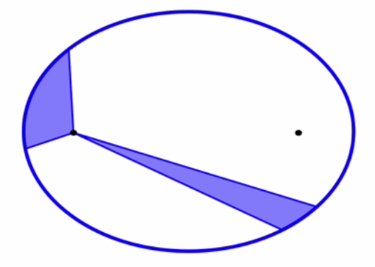
\includegraphics[width=.4\columnwidth]{imagenes/kepler.png}
	\caption{Dibujo esquemático de la segunda ley de Kepler.}
	\label{fig:kepler}
\end{figure}

	\printbibliography[heading=bibintoc]
	
\end{document}